\section{Financial Projections}

\subsection{Five-Year Financial Summary}

\begin{table}[H]
\centering
\begin{tabular}{lrrrrr}
\toprule
\textbf{£'000s} & \textbf{Year 1} & \textbf{Year 2} & \textbf{Year 3} & \textbf{Year 4} & \textbf{Year 5} \\
\midrule
\multicolumn{6}{l}{\textbf{Revenue}} \\
Training Revenue & 150 & 275 & 435 & 580 & 725 \\
Holiday Let Revenue & 25 & 40 & 48 & 55 & 60 \\
Consultancy Revenue & 20 & 35 & 55 & 75 & 95 \\
Online Revenue & 0 & 15 & 45 & 80 & 120 \\
\textbf{Total Revenue} & \textbf{195} & \textbf{365} & \textbf{583} & \textbf{790} & \textbf{1,000} \\
\midrule
\multicolumn{6}{l}{\textbf{Operating Expenses}} \\
Staff Costs & 85 & 145 & 195 & 245 & 295 \\
Facility Costs & 25 & 30 & 35 & 40 & 45 \\
Marketing & 15 & 25 & 35 & 45 & 55 \\
Technology & 20 & 25 & 30 & 35 & 40 \\
Other Operating & 15 & 20 & 25 & 30 & 35 \\
\textbf{Total OpEx} & \textbf{160} & \textbf{245} & \textbf{320} & \textbf{395} & \textbf{470} \\
\midrule
\textbf{EBITDA} & \textbf{35} & \textbf{120} & \textbf{263} & \textbf{395} & \textbf{530} \\
EBITDA Margin & 18\% & 33\% & 45\% & 50\% & 53\% \\
\midrule
Depreciation & 35 & 40 & 45 & 50 & 55 \\
Interest & 12 & 10 & 8 & 6 & 4 \\
\textbf{Net Profit} & \textbf{(12)} & \textbf{70} & \textbf{210} & \textbf{339} & \textbf{471} \\
\bottomrule
\end{tabular}
\end{table}

\subsection{Revenue Growth Analysis}

\begin{center}
\begin{tikzpicture}
\begin{axis}[
    width=\textwidth,
    height=8cm,
    xlabel={Year},
    ylabel={Revenue (£'000s)},
    legend pos=north west,
    ymajorgrids=true,
    grid style=dashed,
    xtick={1,2,3,4,5},
    xticklabels={Year 1, Year 2, Year 3, Year 4, Year 5}
]

% Total Revenue
\addplot[
    color=dreamlab-purple,
    mark=square*,
    line width=2pt
] coordinates {
    (1,195) (2,365) (3,583) (4,790) (5,1000)
};
\addlegendentry{Total Revenue}

% Training Revenue
\addplot[
    color=dreamlab-blue,
    mark=o,
    line width=1.5pt
] coordinates {
    (1,150) (2,275) (3,435) (4,580) (5,725)
};
\addlegendentry{Training}

% Other Revenue
\addplot[
    color=dreamlab-green,
    mark=triangle,
    line width=1.5pt
] coordinates {
    (1,45) (2,90) (3,148) (4,210) (5,275)
};
\addlegendentry{Other Revenue}

\end{axis}
\end{tikzpicture}
\end{center}

\subsection{Capital Requirements}

\subsubsection{Initial Investment Breakdown}

\begin{table}[H]
\centering
\begin{tabularx}{\textwidth}{Xrr}
\toprule
\textbf{Category} & \textbf{Amount (£)} & \textbf{\% of Total} \\
\midrule
\multicolumn{3}{l}{\textbf{Phase 1: Laboratory Setup}} \\
DGX A100 System & 150,000 & 33.3\% \\
GPU Workstations & 60,000 & 13.3\% \\
Network Infrastructure & 25,000 & 5.6\% \\
Lab Fit-out & 35,000 & 7.8\% \\
\midrule
\multicolumn{3}{l}{\textbf{Phase 2: Accommodation}} \\
Property Renovation & 80,000 & 17.8\% \\
Furnishing \& Equipment & 40,000 & 8.9\% \\
Professional Fees & 15,000 & 3.3\% \\
\midrule
\multicolumn{3}{l}{\textbf{Phase 3: Sustainability}} \\
Solar Installation & 35,000 & 7.8\% \\
EV Charging Infrastructure & 10,000 & 2.2\% \\
\midrule
\textbf{Total Capital Required} & \textbf{450,000} & \textbf{100\%} \\
\bottomrule
\end{tabularx}
\end{table}

\subsubsection{Funding Structure}

\begin{center}
\begin{tikzpicture}
    \pie[
        text=legend,
        color={dreamlab-purple, dreamlab-blue, dreamlab-green, dreamlab-orange}
    ]{
        40/Equity Investment (£180k),
        30/Bank Loan (£135k),
        20/Grants (£90k),
        10/Founder Investment (£45k)
    }
\end{tikzpicture}
\end{center}

\subsection{Break-Even Analysis}

\begin{table}[H]
\centering
\begin{tabular}{lrr}
\toprule
\textbf{Metric} & \textbf{Value} & \textbf{Timeline} \\
\midrule
Monthly Fixed Costs & £21,000 & - \\
Variable Cost Ratio & 32\% & - \\
Contribution Margin & 68\% & - \\
Break-even Revenue & £30,882/month & - \\
Break-even Utilisation & 42\% & - \\
\textbf{Expected Break-even} & - & \textbf{Month 14} \\
\bottomrule
\end{tabular}
\end{table}

\subsection{Cash Flow Projections}

\begin{table}[H]
\centering
\begin{tabular}{lrrrrr}
\toprule
\textbf{£'000s} & \textbf{Q1} & \textbf{Q2} & \textbf{Q3} & \textbf{Q4} & \textbf{Year 1} \\
\midrule
Opening Cash & 100 & 65 & 48 & 52 & 100 \\
\midrule
Cash Inflows & 35 & 45 & 55 & 60 & 195 \\
Cash Outflows & (70) & (62) & (51) & (47) & (230) \\
\textbf{Net Cash Flow} & (35) & (17) & 4 & 13 & (35) \\
\midrule
\textbf{Closing Cash} & \textbf{65} & \textbf{48} & \textbf{52} & \textbf{65} & \textbf{65} \\
\bottomrule
\end{tabular}
\end{table}

\subsection{Key Financial Metrics}

\begin{table}[H]
\centering
\begin{tabular}{lrrrrr}
\toprule
\textbf{Metric} & \textbf{Year 1} & \textbf{Year 2} & \textbf{Year 3} & \textbf{Year 4} & \textbf{Year 5} \\
\midrule
Gross Margin & 68\% & 71\% & 73\% & 74\% & 75\% \\
Net Margin & -6\% & 19\% & 36\% & 43\% & 47\% \\
ROI & -3\% & 16\% & 47\% & 75\% & 105\% \\
Payback Period & - & - & 2.8 years & - & - \\
IRR (5-year) & - & - & - & - & 42\% \\
\bottomrule
\end{tabular}
\end{table}

\subsection{Sensitivity Analysis}

\subsubsection{Revenue Sensitivity}

\begin{center}
\begin{tikzpicture}
\begin{axis}[
    xlabel={Revenue Change (\%)},
    ylabel={Net Profit Year 3 (£'000s)},
    grid=major,
    width=0.8\textwidth,
    height=6cm
]
\addplot[
    color=dreamlab-purple,
    mark=*,
    line width=2pt
] coordinates {
    (-20,126) (-10,168) (0,210) (10,252) (20,294)
};
\end{axis}
\end{tikzpicture}
\end{center}

\subsubsection{Key Assumptions and Risks}

\begin{itemize}
    \item \textbf{Utilisation Rate}: Assumes 60\% training capacity by Year 2
    \item \textbf{Price Stability}: No significant price erosion expected
    \item \textbf{Staff Retention}: Key instructor retention critical
    \item \textbf{Technology Refresh}: Major upgrade required Year 4
    \item \textbf{Market Growth}: AI training demand continues expansion
\end{itemize}

\subsection{Return on Investment}

\begin{solarroi}
\textbf{Sustainability Investment Returns}

Solar installation provides both financial and environmental returns:
\begin{itemize}
    \item Annual energy savings: £8,500
    \item Carbon offset: 12 tonnes CO₂/year
    \item Energy independence: 70\% grid reduction
    \item Marketing value: Premium eco-positioning
    \item Total 20-year savings: £215,000
\end{itemize}
\end{solarroi}